% ================================================================
\section{Heaps avançados: binomiais e de Fibonacci}\label{sec:heapav}
% ================================================================
\textbf{Motivação.} No heap binário (vetor) a \textbf{fusão} (união de duas filas) custa $O(n)$: concatena-se os vetores e reconstrói-se com \emph{arranjar}. Em aplicações com muitas fusões (setores de controle, Dijkstra/Prim em grafos grandes) isso é inviável. O heap binomial faz fusão em $O(\log n)$ pior caso; o de Fibonacci, em $O(1)$ amortizado.

% ------------------------------------------------------------------
\subsection{Árvores binomiais}\label{sec:binomial}
\begin{defi}
$B_0$ é um único nó. Para $k\ge1$, $B_k$ é obtida \textbf{subordinando} (\emph{link}) uma $B_{k-1}$ à outra: a raiz de uma vira filho (mais à direita/novo primeiro filho) da raiz da outra. Num heap, a raiz de \emph{maior} prioridade fica por cima.
\end{defi}

\begin{center}
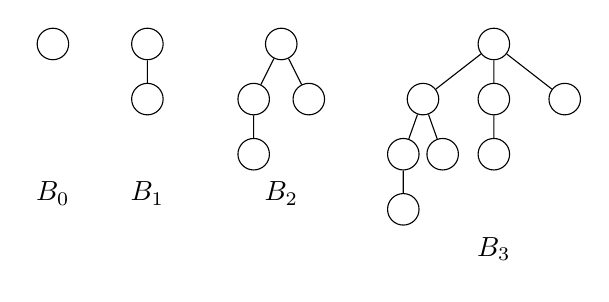
\begin{tikzpicture}[every node/.style={circle,draw,inner sep=1.3pt,minimum size=4mm}, level distance=7mm]
\node (a) at (0,0) {}; \node[draw=none] at (0,-1.9) {$B_0$};
\node (b) at (1.2,0) {} child {node {}}; \node[draw=none] at (1.2,-1.9) {$B_1$};
\node at (2.9,0) {} [sibling distance=7mm] child {node {} child {node{}}} child {node {}}; \node[draw=none] at (2.9,-1.9) {$B_2$};
\node at (5.6,0) {} [sibling distance=9mm] child {node {} [sibling distance=5mm] child {node{} child{node{}}} child{node{}}} child {node {} child{node{}}} child {node {}}; \node[draw=none] at (5.6,-2.6) {$B_3$};
\end{tikzpicture}
\end{center}

\begin{prop}[Propriedades de $B_k$ -- provas por indução em $k$]\label{prop:binom}\leavevmode
\begin{enumerate}
  \item $B_k$ tem exatamente $2^k$ nós \quad($2\cdot2^{k-1}$).
  \item O grau da raiz (a \textbf{ordem} de $B_k$) é $k$, e é o grau máximo da árvore \quad(o link dá mais um filho à raiz).
  \item A altura de $B_k$ é $k$ (medida em arestas) \quad(a subordinada fica um nível abaixo: $\max\{k-1,\,1+(k-1)\}$).
  \item Há exatamente $\binom kj$ nós na profundidade $j$ \quad($\binom{k-1}{j}+\binom{k-1}{j-1}=\binom kj$; daí o nome).
  \item Os filhos da raiz de $B_k$ são raízes de $B_{k-1},B_{k-2},\dots,B_1,B_0$.
\end{enumerate}
\end{prop}

\begin{cuidado}[Convenção de altura: aula $\times$ livro]
Na aula (18/08) e na monitoria ``Heaps Binomiais'': \textbf{$B_k$ tem altura $k$} (conta arestas). No Szwarcfiter e na monitoria ``Heap-fibonacci-binomial'': \textbf{$B_h$ tem altura $h+1$} (conta níveis, folha tem altura 1, como nos heaps binários do curso). É a mesma árvore! Ao responder exercícios de ``alturas'' (lista, ex.\ 8 e 10), \emph{declare a convenção}. Neste resumo: ordem $=$ grau da raiz $=k$ e altura $=k$ arestas.
\end{cuidado}

% ------------------------------------------------------------------
\subsection{Heap binomial}
\begin{defi}
Um \textbf{heap binomial} é uma floresta $H$ de árvores binomiais tal que (1) cada árvore satisfaz a condição de heap (filho $\le$ pai) e (2) as árvores têm \textbf{ordens distintas} (no máximo uma de cada ordem). As raízes ficam numa lista ordenada por ordem crescente.
\end{defi}

\begin{prop}
(a) Para cada $n$ há um único formato de heap binomial com $n$ nós: $B_k\in H$ sse o bit $k$ de $n$ é 1. (b) Logo $H$ tem no máximo $\floor{\log_2 n}+1$ árvores, cada uma de altura $\le\floor{\log_2n}$.
\end{prop}
\begin{proof}
$B_k$ contribui $2^k$ nós e as ordens são distintas, então $n=\sum_{B_k\in H}2^k$ --- é a representação binária de $n$, que é única. Um número $n$ tem $\floor{\log_2 n}+1$ bits.
\end{proof}
\noindent Ex.: $13=1101_2\Rightarrow H=\{B_0,B_2,B_3\}$; $26=11010_2\Rightarrow\{B_1,B_3,B_4\}$.

\subsubsection{Operações}
\begin{pseudo}{Binomial-Link e fusão (Szwarcfiter Alg.\ 9 / monitoria)}
\begin{algorithmic}
\Procedure{Binomial-Link}{$y,z$} \Comment{$y$ e $z$ raízes de $B_{k-1}$; $z$ fica por cima}
  \State $p[y]\gets z$;\quad $sibling[y]\gets child[z]$;\quad $child[z]\gets y$;\quad $degree[z]\gets degree[z]+1$
\EndProcedure
\Procedure{Fusão}{$H',H''$}
  \State $H := H'\cup H''$ \Comment{intercala as listas de raízes por ordem crescente: $O(\log n)$}
  \While{$H$ contém duas árvores $B,B'$ de mesma ordem} \Comment{a menor ordem repetida primeiro}
    \If{$B.raiz.chave \ge B'.raiz.chave$} \State subordinar $B'$ a $B$
    \Else \State subordinar $B$ a $B'$
    \EndIf
  \EndWhile
\EndProcedure
\end{algorithmic}
\end{pseudo}
A fusão é exatamente \textbf{uma soma binária com ``vai um''}: duas $B_k$ viram uma $B_{k+1}$ (o ``vai um''). Como há $O(\log n)$ posições e no máximo 3 árvores de mesma ordem ao mesmo tempo (duas originais + um carry), a fusão custa $O(\log n)$ no pior caso. (Na implementação do Cormen, percorre-se a lista com ponteiros \emph{prev-x}, \emph{x}, \emph{next-x} e há 4 casos: ordens diferentes; três iguais seguidas; dois iguais com $x$ vencendo; dois iguais com \emph{next-x} vencendo.)

\begin{exemplo}[Fusão -- Szwarcfiter Fig.\ 9.10 e exercício da monitoria]
$H_1=\{B_0,B_2,B_4\}$ ($21=10101_2$) e $H_2=\{B_0,B_1\}$ ($3=11_2$). Links na ordem: $B_0+B_0\to B_1$; esse $B_1+B_1$ (de $H_2$) $\to B_2$; esse $B_2+B_2$ (de $H_1$) $\to B_3$. Resultado $\{B_3,B_4\}$, isto é, $24=11000_2=10101_2+11_2$.
\end{exemplo}

\begin{itemize}
  \item \textbf{Inserção:} fusão com um heap $\{B_0\}$ contendo só o novo nó. Pior caso $O(\log n)$ (quando $n=2^k-1$, todos os bits são 1 e há $k$ links). \emph{Tempo esperado $O(1)$} (Lema 9.3 do Szwarcfiter: se $j$ é a posição do primeiro 0 de $n$ em binário, lida da direita para a esquerda, a inserção faz $j$ ``fusões'' no sentido do livro, das quais $j-1$ são links, um por 1 final de $n$; com bits equiprováveis, $E[j]=\sum_{j\ge1}j/2^j=2$, isto é, 2 passos esperados e 1 link esperado) e \emph{amortizado $O(1)$} (dá-se 1 crédito a cada árvore; cada link é pago pelo crédito da árvore subordinada, que some --- é o contador binário).
  \item \textbf{Seleção do máximo:} o máximo é uma das $\le\floor{\log n}+1$ raízes: $O(\log n)$, ou $O(1)$ mantendo um ponteiro para a maior raiz (atualizado nas operações).
  \item \textbf{Remoção do máximo:} ache a raiz $r$ máxima, numa árvore $B_k$; retire $B_k$ de $H$ ($H'=H-B_k$); retirando $r$, seus filhos $B_{k-1},\dots,B_0$ formam um heap binomial $H''$; faça a fusão $H'\cup H''$. Total $O(\log n)$.
  \item \textbf{Alteração de prioridade:} \emph{aumentar} $\Rightarrow$ sobe dentro da própria árvore trocando com o pai, como no heap binário: $O(\log n)$ (altura $\le\log n$). \emph{Diminuir} $\Rightarrow$ remover o nó (ver abaixo) e reinseri-lo com a nova prioridade: $O(\log n)$. (Descer trocando com o maior filho também funciona, mas cada nível tem até $O(\log n)$ filhos para comparar: $O(\log^2 n)$.)
  \item \textbf{Remoção de um nó qualquer:} aumente sua prioridade para $+\infty$ (sobe até a raiz) e remova o máximo: $O(\log n)$.
  \item \textbf{Construção:} $n$ inserções custam $O(n)$ no total (contador binário: $\sum_k n/2^k\le 2n$). É a resposta do ex.\ 7 da lista.
\end{itemize}

% ------------------------------------------------------------------
\subsection{Heap de Fibonacci}\label{sec:fib}
\textbf{Ideia: preguiça.} O heap binomial é ``estrito'': toda inserção/fusão já resolve colisões de ordem. O de Fibonacci \emph{adia} toda a arrumação para a remoção do máximo.

\paragraph{Estrutura.} Floresta de árvores com condição de heap; as raízes numa \textbf{lista circular duplamente encadeada}, e os filhos de cada nó também. Ponteiro para a raiz máxima. Cada nó guarda: chave, pai, um filho, irmãos esquerdo/direito, grau, e um bit \textbf{marca}. Listas circulares duplas permitem inserir/remover um nó ou concatenar duas listas em $O(1)$.

\paragraph{Operações} (heap de máximo, como no curso; ``aumentar prioridade'' = \emph{decrease-key} do Cormen, que usa heap de mínimo).
\begin{itemize}
  \item \textbf{Inserção:} cria uma árvore de um nó e a coloca na lista de raízes; atualiza o ponteiro do máximo. $O(1)$ real.
  \item \textbf{Fusão:} concatena as duas listas de raízes; máximo $=$ maior dos dois. $O(1)$ real.
  \item \textbf{Seleção:} ponteiro. $O(1)$.
  \item \textbf{Remoção do máximo:} (1) remove a raiz máxima e promove todos os seus filhos a raízes (desmarcados); (2) \textbf{consolida}: percorre as raízes com um vetor $A[0..D]$ indexado pelo grau ($D=O(\log n)$); sempre que duas raízes têm o mesmo grau, subordina a de menor prioridade à de maior (o grau sobe de 1) e repete; (3) reconstrói a lista de raízes a partir de $A$ e acha o novo máximo. Real: $O(D+t)$ com $t=$ número de raízes; \textbf{amortizado $O(\log n)$}.
  \item \textbf{Aumento de prioridade de $x$:} aumenta a chave; se não ficou maior que o pai, fim. Senão: \textbf{corta} $x$ (com sua subárvore) e o põe na lista de raízes, desmarcado; então, subindo: se o pai $y$ está \emph{desmarcado}, marque-o (se não for raiz) e pare; se $y$ já estava \emph{marcado} (perdeu um filho antes), corte $y$ também, desmarque-o, leve-o à lista de raízes e continue com o pai de $y$ --- \textbf{cortes em cascata}. \textbf{Amortizado $O(1)$}.
  \item \textbf{Remoção de nó qualquer:} aumenta para $+\infty$ e remove o máximo: $O(\log n)$\am.
  \item \textbf{Diminuição de prioridade:} não é a operação ``barata''; faz-se removendo e reinserindo (ou cortando os filhos que passarem a violar): $O(\log n)$\am. Na tabela da aula (convenção de mínimo), isso aparece como ``incrementar $O(\log n)$\am, decrementar $O(1)$\am''.
\end{itemize}

\paragraph{Regras das marcas.} Todos começam desmarcados; um nó é marcado quando \emph{perde o primeiro filho} por corte; ao perder o segundo, ele próprio é cortado. \textbf{Raízes nunca estão marcadas} (e podem perder vários filhos); ao ser subordinado a outro nó, o nó fica desmarcado.

\begin{exemplo}[Cortes em cascata -- exercício da monitoria de 26/08]
Nó interno $X$ com pai $Y$ (marcado) e avô $Z$ (marcado); a prioridade de $X$ aumenta violando a ordem. (1) $X$ é cortado e vai para a lista de raízes (desmarcado). (2) $Y$ perdeu seu segundo filho: é cortado, desmarcado, vai para a lista de raízes. (3) Idem para $Z$. (4) Seja $W$ o pai de $Z$: se $W$ é raiz, nada muda; se não é raiz e está desmarcado, passa a \textbf{marcado} e a cascata para; se estava marcado, a cascata continua. Nós movidos para as raízes: $X,Y,Z$ (e possivelmente mais); flags: $X,Y,Z$ desmarcados, $W$ marcado (se não raiz).
\end{exemplo}

\subsubsection{Por que funciona: grau máximo $O(\log n)$}
\begin{lema}
Seja $x$ um nó e $y_1,\dots,y_k$ seus filhos na ordem em que foram ligados a $x$. Então $\operatorname{grau}(y_i)\ge i-2$.
\end{lema}
\begin{proof}
Quando $y_i$ foi ligado, $x$ já tinha $y_1,\dots,y_{i-1}$, logo grau $\ge i-1$; só se ligam nós de mesmo grau, então $y_i$ tinha grau $\ge i-1$. Desde então $y_i$ perdeu no máximo um filho (senão teria sido cortado). Logo $\operatorname{grau}(y_i)\ge i-2$.
\end{proof}
\begin{teo}
Um nó de grau $k$ tem subárvore com pelo menos $F_{k+2}\ge\varphi^k$ nós ($F$ = Fibonacci, $\varphi=\frac{1+\sqrt5}2$). Logo o grau máximo é $D(n)\le\log_\varphi n=O(\log n)$, e um heap de Fibonacci tem $O(\log n)$ árvores após a consolidação.
\end{teo}
\begin{proof}[Esboço]
Seja $s_k$ o tamanho mínimo de uma subárvore de raiz com grau $k$. Pelo lema, $s_k\ge 2+\sum_{i=2}^{k}s_{i-2}$, e por indução $s_k\ge F_{k+2}$ (pois $F_{k+2}=1+\sum_{i=0}^{k}F_i$). É daí que vem o nome: as menores árvores de posto $k$ ($F_0,\dots,F_5$ desenhadas em aula) têm $1,2,3,5,8,13$ nós.
\end{proof}
\noindent Sem marcas/cascata, poderíamos cortar todos os netos de uma raiz: uma árvore de posto $k$ com só $k+1$ nós; o posto deixaria de ser $O(\log n)$ e a consolidação ficaria cara (resposta ao ``Exercício 3'' da monitoria).

\subsubsection{Análise amortizada}
Potencial (Cormen, cap.~19): $\Phi(H)=t(H)+2\,m(H)$, com $t=$ nº de raízes e $m=$ nº de nós marcados.
\begin{itemize}
  \item Inserção: real $O(1)$, $\Delta\Phi=+1$ $\Rightarrow O(1)$. Fusão: $\Delta\Phi=0$ $\Rightarrow O(1)$.
  \item Remoção do máximo: real $O(D+t)$; depois há $\le D+1$ raízes, então $\Delta\Phi\le (D+1)-t$ $\Rightarrow$ amortizado $O(D)=O(\log n)$. \emph{O custo de consolidar as $t$ raízes acumuladas foi ``pago'' pelas inserções/fusões preguiçosas.}
  \item Aumento de prioridade com $c$ cortes em cascata: real $O(c)$; $t$ cresce $c$, $m$ cai $\ge c-2$ $\Rightarrow\Delta\Phi\le c+2(2-c)=4-c$ $\Rightarrow$ amortizado $O(1)$. (Visão do banqueiro do Szwarcfiter: o corte de um nó marcado é debitado à operação que o marcou.)
\end{itemize}
\begin{teo}[Aula de 21/08]
A partir de um heap de Fibonacci vazio, qualquer sequência de $a_1$ inserções, $a_2$ remoções, $a_3$ aumentos de prioridade e $a_4$ uniões custa $O(a_1+a_3+a_4+a_2\log n)$.
\end{teo}

\begin{cuidado}
\begin{itemize}
  \item Os $O(1)$ do Fibonacci são \textbf{amortizados}: \emph{uma} remoção do máximo após muitas inserções/fusões pode custar $\Theta(n)$ (consolida tudo de uma vez). Se o requisito é previsibilidade de cada operação, Fibonacci é ruim.
  \item Constantes grandes e muita memória por nó (4 ponteiros + grau + marca): na prática só compensa com MUITAS alterações de prioridade (Dijkstra/Prim em grafos densos).
  \item Uma árvore de um heap de Fibonacci \emph{pode} ter altura grande (até $\Theta(n)$ em sequências adversárias; Cormen, ex.~19.4-1): o que é logarítmico é o \textbf{grau}, não a altura.
\end{itemize}
\end{cuidado}

% ------------------------------------------------------------------
\subsection{Comparação e escolha da estrutura (Q4 e Teste 1)}\label{sec:escolhaheap}
\begin{center}
\small
\begin{tabular}{@{}l>{\centering\arraybackslash}p{3.3cm}>{\centering\arraybackslash}p{4.2cm}>{\centering\arraybackslash}p{3.6cm}@{}}
\toprule
& Heap binário & Heap binomial & Heap de Fibonacci\\
\midrule
Seleção & $O(1)$ & $O(\log n)$ / $O(1)$ c/ ponteiro & $O(1)$\\
Inserção & $O(\log n)$ & $O(\log n)$ pior; $O(1)$ esp./amort. & $O(1)$\am\\
Remoção do máx. & $O(\log n)$ & $O(\log n)$ & $O(\log n)$\am\\
Aumentar prioridade & $O(\log n)$ & $O(\log n)$ & $O(1)$\am\\
Fusão & $O(n)$ & $O(\log n)$ \textbf{pior caso} & $O(1)$\am\\
Construção & $O(n)$ & $O(n)$ & $O(n)$\\
Memória & vetor, sem ponteiros & 3 ponteiros + grau/nó & 4 ponteiros + grau + marca/nó\\
Garantia & pior caso & pior caso & amortizada\\
Simplicidade & muito simples & média & complexa\\
\bottomrule
\end{tabular}
\end{center}

\begin{prova}[Roteiro de escolha]
\begin{enumerate}
  \item Precisa de \textbf{fusão}? Não $\Rightarrow$ \textbf{heap binário} (mais simples, menos memória, ótimo em cache).
  \item Fusão frequente e \textbf{cada operação precisa ser previsível} (limite de tempo por operação, sistema de tempo real) $\Rightarrow$ \textbf{heap binomial} (fusão $O(\log n)$ \emph{pior caso}).
  \item Muitíssimos \textbf{aumentos de prioridade} (ou fusões) e o que importa é o \textbf{custo total} da execução $\Rightarrow$ \textbf{heap de Fibonacci}.
  \item Restrição de \textbf{memória} forte $\Rightarrow$ binário (as outras têm overhead de ponteiros por nó).
\end{enumerate}
\end{prova}

\paragraph{Teste 1 -- respostas esperadas.}
\begin{itemize}
  \item \textbf{Q1 (aeroporto):} fusões muito frequentes com filas de centenas de milhares de aeronaves; alterações raras; exigência de tempo \emph{previsível por operação individual}. $\Rightarrow$ \textbf{Heap binomial}: fusão em $O(\log n)$ no pior caso de \emph{cada} execução, crescendo só logaritmicamente. Binário: fusão $O(n)$ (reconstrução) --- milhares de fusões com $10^5$ elementos estouram a janela. Fibonacci: fusão $O(1)$ só \emph{amortizada}; o custo acumulado aparece de uma vez numa remoção (consolidação $\Theta(n)$ possível) --- imprevisível; e sua vantagem (aumento de prioridade $O(1)$) não é usada, pois alterações são raras.
  \item \textbf{Q2 (central médica, 40 MB):} $2\cdot10^6$ chamadas $\times$ 16 bytes $=32\,000\,000$ bytes $\approx 30{,}5$ MB $<41\,943\,040$. Heap binomial precisaria de $\ge3$ ponteiros (pai, filho, irmão $=24$ bytes) $+$ grau: $\ge 40$ bytes/nó $\Rightarrow\ge 80\cdot10^6$ bytes; Fibonacci ($\ge4$ ponteiros $+$ grau $+$ marca) ainda mais. Não há fusão, alterações são poucas, inserção/remoção $O(\log n)$ bastam. $\Rightarrow$ \textbf{Heap binário em vetor} (único que cabe, e o mais simples).
  \item \textbf{Q3 (supercomputador):} $5\cdot10^6$ inserções, $5\cdot10^6$ remoções, $80\cdot10^6$ aumentos de urgência, poucas uniões; importa o custo total. Fibonacci: $\approx 5\cdot10^6+80\cdot10^6+5\cdot10^6\log_2(5\cdot10^6)\approx 2\cdot10^8$ passos; binário/binomial: $\approx 90\cdot10^6\cdot 22\approx 2\cdot10^9$. $\Rightarrow$ \textbf{Heap de Fibonacci} (aumento $O(1)$\am\ sem remover/reinserir). Binário/binomial pagam $O(\log n)$ em cada um dos 80 milhões de aumentos.
\end{itemize}
